
\chapter{Synthetic data sets}

\index{synthetic data set}

Last chapter we learned the basic skills for generating arrays of random values
-- both numeric and categorical. Now let's apply these to creating
\textbf{synthetic data set}s that contain more than one variable.

We'll concentrate here on the two-variable case, but the idea is easily
extended to three or more. The important new question, now that we know how to
generate single arrays in isolation, is: to what degree do we want our pair
of synthetic variables to be correlated, and how do we make them so?

\section{\textit{Numeric} variables}

\index{association}
\index{Pearson correlation coefficient}
\index{correlation coefficient}
\index{p-value@$p$-value}

Let's start with the case of two numeric variables. As you know from DATA 101,
there can be an association, or not, between them. The Pearson's correlation
coefficient measures this: if its $p$-value is less than our $\alpha$ setting
(typically .05), then we deem there to be a meaningful association, and the $r$
value tells us whether the correlation is positive or negative.

\subsection{Uncorrelated numeric variables}

On one extreme, let's say you wanted to create a data set with two completely
\textit{uncorrelated} numeric variables -- like the heights (in inches) and the
SAT scores of a group of college applicants. Then you'd just generate two
arrays, one at a time:

\index{sat\_scores@\texttt{sat\_scores}}
\index{heights@\texttt{heights}}

\begin{Verbatim}[fontsize=\small,samepage=true,frame=single]
heights = np.random.normal(65, 8, 100)
sat_scores = np.random.normal(1000, 300, 100)
\end{Verbatim}

\index{Pearson correlation coefficient}
\index{correlation coefficient}
\index{pearsonr@\texttt{pearsonr()} (SciPy)}

How did I choose those particular means and standard deviations? I made them
up. And I played with them until they looked reasonable.

Scatter plotting these (see left side of Figure~\ref{uncorrscatter},
p.~\pageref{uncorrscatter}), and running a Pearson correlation, should reveal
they are independent of each other:

\begin{Verbatim}[fontsize=\small,samepage=true,frame=single,framesep=3mm]
plt.scatter(heights, sat_scores)
plt.xlabel("height (in)")
plt.ylabel("SAT score")
print(scipy.stats.pearsonr(heights,sat_scores))
\end{Verbatim}
\vspace{-.2in}

\begin{Verbatim}[fontsize=\small,samepage=true,frame=leftline,framesep=5mm,framerule=1mm]
(-0.025053425275878834, 0.8045806864145338)
\end{Verbatim}

A $p$-value of .8046 says ``nope, not significantly correlated.'' And of course
there's no reason why they should be: we just generated two different random
arrays, for different ranges.

Incidentally, you might be troubled by the fact that a few of our SAT scores
are outside the legal range:

\begin{Verbatim}[fontsize=\small,samepage=true,frame=single,framesep=3mm]
print("min: {}, max: {}".format(sat_scores.min(), sat_scores.max()))
\end{Verbatim}
\vspace{-.2in}

\begin{Verbatim}[fontsize=\small,samepage=true,frame=leftline,framesep=5mm,framerule=1mm]
min: 304.29, max: 1618.35
\end{Verbatim}

\index{clip@\texttt{.clip()} method (NumPy)}

Real SAT scores are supposed to range between 400 and 1600, the Internet tells
me. We could fix this by using the NumPy \texttt{.clip()} method, which imposes
a high and low cutoff as its arguments:

\begin{Verbatim}[fontsize=\small,samepage=true,frame=single,framesep=3mm]
sat_scores = sat_scores.clip(400,1600)
print("min: {}, max: {}".format(sat_scores.min(), sat_scores.max()))
\end{Verbatim}
\vspace{-.2in}

\begin{Verbatim}[fontsize=\small,samepage=true,frame=leftline,framesep=5mm,framerule=1mm]
min: 400.0 max: 1600.0
\end{Verbatim}

The revised scatter plot is shown on the right side of Figure~\ref{uncorrscatter}.

\begin{figure}[ht]
\centering
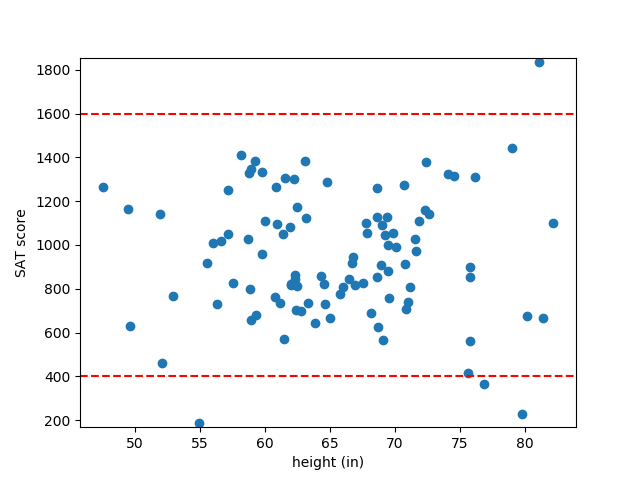
\includegraphics[width=0.45\textwidth]{uncorrscatter.png}
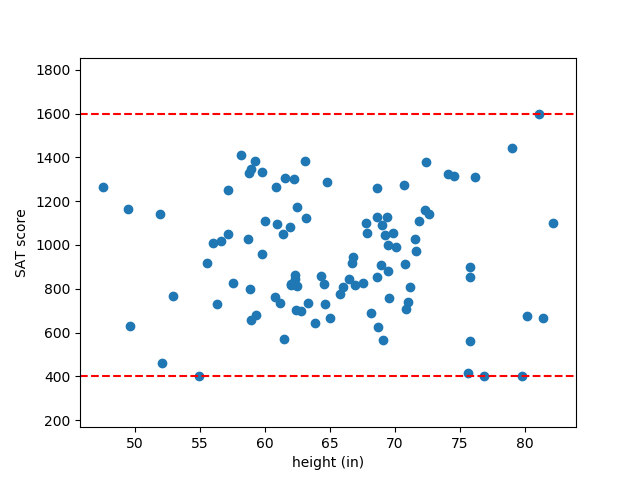
\includegraphics[width=0.45\textwidth]{uncorrscatterclip.png}
\smallskip
\caption{Uncorrelated numeric random variables. The right-hand plot has SAT
scores ``clipped'' to stay above 400 and below 1600.}
\label{uncorrscatter}
\end{figure}



\subsection{Totally correlated numeric variables}

On the other extreme, if two variables are \textit{completely} correlated, then
one is simply a direct (linear) function of the other. That's easy to
accomplish by creating only \textit{one} randomly, and then using it to compute
the other:

\begin{Verbatim}[fontsize=\small,samepage=true,frame=single]
weights_lbs = np.random.normal(150, 30, 100)
weights_kg = weights_lbs / 2.2
\end{Verbatim}

Clearly a person's weight in pounds completely determines their weight in
kilograms: all you do is divide by a constant factor to convert between units.

\begin{figure}[ht]
\centering
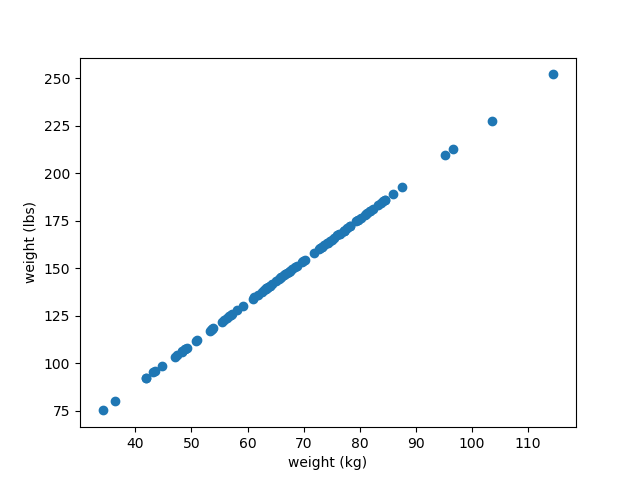
\includegraphics[width=0.45\textwidth]{compcorrscatter.png}
\smallskip
\caption{Two \textit{completely} correlated numeric variables.}
\label{compcorrscatter}
\end{figure}

Scatter plotting these gives a perfectly straight line (see
Figure~\ref{compcorrscatter}), and Pearson tells us they're totally correlated
(the $p$-value is rock bottom 0.0, and $r$=1):

\index{pearsonr@\texttt{pearsonr()} (SciPy)}

\begin{Verbatim}[fontsize=\small,samepage=true,frame=single,framesep=3mm]
print(scipy.stats.pearsonr(weights_lbs,weight_kg))
\end{Verbatim}
\vspace{-.2in}

\begin{Verbatim}[fontsize=\small,samepage=true,frame=leftline,framesep=5mm,framerule=1mm]
(1.0, 0.0)
\end{Verbatim}

\subsection{Somewhat correlated numeric variables}

Now let's take the most common and interesting case: a data set in which our
two numeric variables are \textit{partially}, but not completely, correlated.
(By ``partially correlated'' I just mean that there \textit{is} an association
between the variables, but it's not a rigidly perfect one, like the one between
weight-in-pounds and weight-in-kg.)

\index{noise}

What we'll do is first generate one of the variables independently and
randomly, and then compute the second as a function of the first \textit{with
added \textbf{noise}}. ``Noise'' is a strange (and somewhat misleading) term
that's used in a variety of statistical situations. Here it means ``random
other factors that influence a numeric variable's value up or down.''

\index{SAT}
\index{GPA}

As an example, let's create a synthetic data set with two variables about high
school seniors: her SAT score, and her high school GPA. A moment's thought
will tell you that this indeed falls under our third, ``somewhat correlated''
case: students with better SAT scores also on average tend to have higher GPAs,
but this is an imperfect relationships that doesn't always hold completely.

\index{nudge@``nudge''}

Our strategy is as follows. First, randomly create an array of synthetic SAT
scores. Then, calculate each student's GPA as a function of her SAT score,
plus a random ``nudge'' either up or down to account for other random factors.

\index{white noise}

For our noise factor (the ``nudge'') we'll take the most common approach: a
normally-distributed random variable with a mean of zero. This is called
``\textbf{white noise},'' for various semi-interesting reasons. We use a mean
of 0 for this because on average, we don't want the random ``nudges'' to be
biased in either the up direction or the down direction. On average, we want
the net nudge to be zero.

Okay. Now see if you can understand the two lines of code we use to implement
this strategy:

\index{sat\_scores@\texttt{sat\_scores}}

\begin{Verbatim}[fontsize=\small,samepage=true,frame=single,framesep=3mm]
sat_scores = np.random.normal(1000, 300, 100)
gpas = sat_scores * (2.5 / 1400) + np.random.normal(0, 1, 100)
\end{Verbatim}

The \texttt{sat\_scores} line is the same one we had before. We're then
modeling the high school GPA of a student as \textit{somewhat} correlated with
his SAT score. The ``$\frac{2.5}{1400}$'' multiplier is an attempt to quantify
the relationship between the two variables, which of course are measured on
completely different scales. We're guestimating that a 1400 on the SAT would
kinda sorta equate to about a 2.5 GPA. Notice that the second component of
\texttt{gpas} is a normally distributed noise component \textit{with zero
mean}. (Why a standard deviation of 1? Just a guess. We can tweak it later if
we don't like the results.)

Now this is a good first attempt. Notice two assumptions/limitations, though:

\begin{enumerate}

\item We're assuming that the relationship between the two variables is
\textit{linear} --- namely, that ``the first value times a constant'' is a good
estimate for the second value. In reality, of course, the relationship is often
more complex: it might be better modeled as the \textit{square} of the first
value, for instance, or ``$e$ to the'' first value, or the cube root of the
first value, \textit{etc.}

\index{intercept term}

\item We're assuming that the ``zero point'' for the two variables coincide: in
other words, a zero for one value would on average roughly correspond to a zero
for the other. In the above case, we're assuming that a person who got a 0 on
the SAT would have, on average, a 0 GPA. If this isn't appropriate, we should
add an \textbf{intercept term} (a constant) to our generative formula. This
takes our generated second variable and just shifts it, wholesale, to a new
region of the number range.

\end{enumerate}

We'll stick with the first assumption (linearity) for the moment, but be more
flexible about the second. If we include an intercept term, our formula for
generating the dependent variable boils down to:

\begin{center}

\texttt{dep\_variable} = $m \ \cdot$ \texttt{indep\_variable} + $b$ +
\texttt{np.random.normal(0, $\sigma$, $n$)}

\end{center}

\index{y=mx+b@$y=mx+b$}

which is the familiar equation for a line ($y=mx+b$) with a noise term added
in (with $\sigma$ standard deviation). Now we have to estimate decent values
for $m$, $b$, and $\sigma$. How should we do this?

\medskip

My preferred approach is to identify a ``high-ish'' value of the first
variable, and estimate a (roughly, on average) corresponding value of the
second variable. Then do the same for a ``low-ish'' value. Then, plug those
into the $y=mx+b$ formula and solve for the slope and intercept.

Example: let's generate a synthetic data set of two variables: the number of
hours a person has practiced playing the Dance Dance Revolution (DDR) videogame
in their lifetime, and the score they achieved in a DDR contest (on the song
\textit{Kakumei}). Clearly, there should be some (positive) relationship
between the two quantities: when \texttt{num\_hrs} is high, you'd expect
\texttt{score} to also be high. If you're familiar with the game, though, you
know that the zero points for these variables do \textit{not} coincide: even if
you've never ever played at all, you'll still manage to stumble through the
song, learn how to play as you go, and get a positive score.

Based on my knowledge of the game (which I suck at, by the way), I estimate: 

\begin{compactitem}

\item A decent player who has practiced for 100 hours might get a score of
around 60 million.
%\footnote{For whatever reason, even bad scores in DDR are
%zany high numbers. To avoid writing out tons of zeros, I'll just consider
%``60'' to be a player's score instead of ``60,000,000.''}

\item A sucky-ish player who has practiced for only 10 hours might
get a score of around 30 million.

\end{compactitem}


Running the algebra\footnote{Linear algebra fans can avoid doing all the
mechanical steps by noting that our two equations form the following matrix
equation:
\vspace{-.2in}

\begin{align*}
\begin{bmatrix} 100 & 1 \\ 10 & 1 \end{bmatrix}
\cdot
\begin{bmatrix} m \\ b \end{bmatrix}
=
\begin{bmatrix} 60 \\ 30 \end{bmatrix}
\end{align*}

NumPy can solve this for $m$ and $b$ like so:

\begin{Verbatim}[fontsize=\small,samepage=true,frame=single,framesep=3mm]
X = np.array([[100,1],[10,1]])
Y = np.array([60,30])
print(np.linalg.solve(X,Y))
\end{Verbatim}
\vspace{-.2in}

\begin{Verbatim}[fontsize=\small,samepage=true,frame=leftline,framesep=5mm,framerule=1mm]
[ 0.33333333 26.66666667]
\end{Verbatim}
But only if you're feeling lazy. 
}, I get:
\begin{samepage}
\begin{align*}
60 &= m \cdot 100 + b\\
30 &= m \cdot 10 + b\\
\end{align*}
\vspace{-.7in}
\begin{center}
\dots \textit{insert algebra here} \dots \\
\smallskip
$m = .333, b = 26.667$
\end{center}
\end{samepage}

Thus we get back-of-the-envelope estimates of $m$ and $b$.

Now how to estimate $\sigma$, the standard deviation of the noise term? Play
with it. The larger it is, the more your second variable will deviate from the
perfectly straight line we would predict solely from the $y=mx+b$. Remember
that with the normal distribution, two-thirds of your data points will fall
within one standard deviation from the mean. I think two-thirds of my 100-hour
practicers might get between 50 and 70 million. So I'll go with a
$\sigma$ of 10 and see how that looks.

Finall, here's the actual code to produce a synthetic data set of 200 dancers.
First, generate the practice times themselves:

\index{clip@\texttt{.clip()} method (NumPy)}

\begin{Verbatim}[fontsize=\small,samepage=true,frame=single,framesep=3mm]
num_hrs = np.random.normal(50,20,200).clip(0,500)
\end{Verbatim}

Perhaps your average dancer practiced 50 hours for the competition, with most
of them within 20 hours of that, and no one who practiced less than 0 hours
(not even me), or greater than 500 hours.

Then, we generate these players' scores:

\begin{Verbatim}[fontsize=\small,samepage=true,frame=single,framesep=3mm]
score = num_hrs * .333 + 26.667 + np.random.normal(0,10,200)
\end{Verbatim}

I think it looks pretty decent (Figure~\ref{ddr}).

\begin{figure}[ht]
\centering
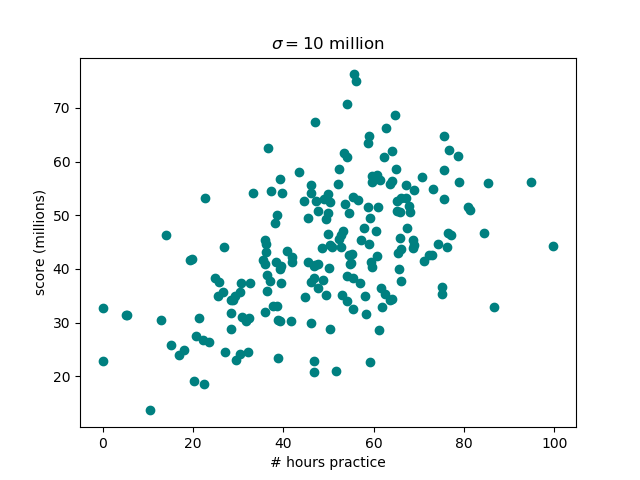
\includegraphics[width=0.46\textwidth]{ddr1.png}
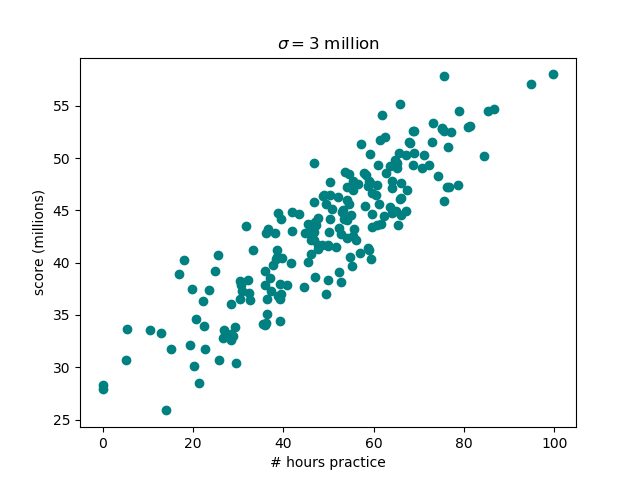
\includegraphics[width=0.46\textwidth]{ddr2.png}
\caption{A scatter plot of two synthetic, partially-but-not-completely
correlated numeric variables. In the left figure, the $\sigma$ for the noise
was set to 10 million; in the right, to 3 million.}
\label{ddr}
\end{figure}

Note: there's also a \texttt{multivariate\_normal()} function in the
\texttt{scipy.stats} package which can generate these kinds of correlated data
sets more powerfully.


%\section{\textit{Categorical} variables}
%
%NumPy provides a way to generate a categorical data set with certain
%frequencies, through its \texttt{np.random.choice()} function:
%
%\begin{Verbatim}[fontsize=\small,samepage=true,frame=single] >>>
%np.random.choice(['Steelers','Redskins','Giants']) 'Redskins' \end{Verbatim}
%
%Useful arguments include:
%
%\begin{compactitem} \item \texttt{size} -- the number of elements you want in
%the resulting array. \item \texttt{replace} -- if \texttt{False}, the elements
%will be drawn from your list \textit{without replacement} (meaning once a
%value is chosen, it will not be chosen again). This is often useful. \item
%\texttt{p} -- a list of \textit{probabilities} (in the range 0 to 1)
%specifying how likely each element in the list is to be chosen. (Note these
%must sum to 1; and NumPy, stupidly, will not normalize it for you.)
%\end{compactitem}
%
%A more complicated example:
%\begin{Verbatim}[fontsize=\footnotesize,samepage=true,frame=single] >>>
%np.random.choice(['Steelers','Redskins','Giants'], size=10, p=[.3,.6,.1])
%['Redskins' 'Redskins' 'Giants' 'Redskins' 'Redskins' 'Steelers' 'Redskins'
%'Steelers' 'Redskins' 'Giants'] \end{Verbatim}
%
%
%\subsection{Uncorrelated categorical variables}
%
%Let's generate a data set with 2000 registered voters in Fredericksburg, 54\%
%Democrats and 46\% Republicans. We'll also generate their pick for the
%Superbowl: Eagles (30\%) or Patriots (70\%).
%
%Since these variables are uncorrelated, we generate each one separately:
%
%\begin{Verbatim}[fontsize=\footnotesize,samepage=true] party =
%np.random.choice(['Democrat','Republican'], p=[.54,.46], size=2000) superbowl
%= np.random.choice(['Eagles','Patriots'], p=[.3,.7], size=2000) \end{Verbatim}
%
%As expected, a $\chi^2$ test's p-value shows no correlation:
%
%\begin{Verbatim}[fontsize=\footnotesize,samepage=true] >>>
%pd.crosstab(superbowl,party) Democrat  Republican Eagles         334 286
%Patriots       746         634
%
%>>> round(scipy.stats.chi2_contingency(pd.crosstab(superbowl,party))[1],2)
%0.98 \end{Verbatim}
%
%\subsection{Completely correlated categorical variables}
%
%Now let's add a ``\texttt{party\_color}'' categorical variable that gives the
%associated color of each voter's political party (blue for Democrats and red
%for Republicans). Since this is perfectly correlated with \texttt{party}, we
%can generate another vector from scratch with the same setup. The
%\texttt{np.where()} function comes in handy:
%
%\begin{Verbatim}[fontsize=\footnotesize,samepage=true] party_color =
%np.where(party=='Democrat','blue','red') \end{Verbatim}
%
%\texttt{np.where()} is tricky but powerful. It takes three arguments -- a
%vector of booleans (\texttt{True}s and \texttt{False}s), and two other
%arguments which are used as substitutions. It produces a vector \textit{that
%includes the second argument in every position where the first is
%\texttt{true}, and the third argument everywhere it's \texttt{false}.} In the
%current example, we're saying ``for every place that the \texttt{party} vector
%has a \texttt{\textquotesingle Democrat\textquotesingle } value, put
%\texttt{\textquotesingle blue\textquotesingle } in this new vector you're
%making for me, and put \texttt{\textquotesingle red\textquotesingle }
%everywhere else.''
%
%We thus (obviously) get perfect correlation:
%
%\begin{Verbatim}[fontsize=\footnotesize,samepage=true] In [30]:
%pd.crosstab(party,party_color) Out[30]: blue  red Democrat    1080    0
%Republican     0  920
%
%>>> round(scipy.stats.chi2_contingency(pd.crosstab(party, party_color))[1],2)
%0.0 \end{Verbatim}
%
%\subsection{Somewhat correlated categorical variables}
%
%Finally, let's create a ``\texttt{gun\_owner}'' categorical variable which has
%the value \texttt{True} or \texttt{False} for each voter: it should be true
%for roughly 44\% of Republicans and for 20\% of Democrats. For this, we can go
%back to our friend \texttt{np.where()}:
%
%\begin{Verbatim}[fontsize=\footnotesize,samepage=true] gun_owner =
%np.where(party=='Democrat',
%np.random.choice([True,False],p=[.2,.8],size=2000),
%np.random.choice([True,False],p=[.44,.56],size=2000)) \end{Verbatim}
%
%This time, our second and third arguments to \texttt{np.where()} are
%\textit{vectors themselves}. We're saying, ``in every position where
%\texttt{party} has a \texttt{\textquotesingle Democrat\textquotesingle }, use
%the corresponding value from our random vector that is 80\% \texttt{false}s.
%Otherwise, use the corresponding value from a different random vector that is
%56\% \texttt{false}s.''
%
%Checking, we do get the desired correlation:
%
%\begin{Verbatim}[fontsize=\footnotesize,samepage=true] >>
%pd.crosstab(party,gun_owner) False  True Democrat      841    239 Republican
%505    415
%
%>> scipy.stats.chi2_contingency(pd.crosstab(party,gun_owner))[1]
%1.5994151557508934e-27 \end{Verbatim}
